\section{Pose Estimation}  \label{sec:pose}
The sensor readings from a smartphone measure the physical quantity in the local coordinate system of the phone, e.g., the acceleration components along the phone's width, length and depth directions ($x', y'$ and $z'$ as shown in Figure~\ref{pix:coordinates}). Because in most cases the phone's axes are not exactly aligned with respective axes of the vehicle, a transformation is needed to derive the acceleration or attitude angles of the vehicle from those of the phone.

In this section, we describe how to estimate the directions of the vehicle's axes ($(x, y, z)$ in Figure~\ref{pix:coordinates}) in the phone's coordinate system. First, we find the direction of the vehicle's $z$ axis from the gravity, assuming that the vehicle is on a level surface. Next we detect the direction of the vehicle's $y$ axis from its acceleration and de-acceleration when moving along straight lines. After $y$ and $z$ axes are decided, the $x$ axis is determined in the phone's coordinate system as well.

%acceleration and cannot be directly used if coordinate systems of the vehicle and the smartphone do not coincide, which happens in most real world cases. As illustrated in Figure~\ref{pix:coordinates}, $(x, y, z)$ represent the coordinates of the vehicle, and $(x', y', z')$ represent the coordinates of the smartphone. In this section, we describe the method to estimate the direction of $(x, y, z)$, which we called \textit{pose} in this paper, regarding the coordinates system of the smartphone as a reference system. First, we choose the opposite direction of the gravity to be z-axis. Second, we estimate the y-axis position on the xy-plane of the vehicle during its straight driving. Finally, we derive the direction distribution of the y-axis instead of a fixed direction when the vehicle is moving forward.
\begin{figure}[h]
  \centering
  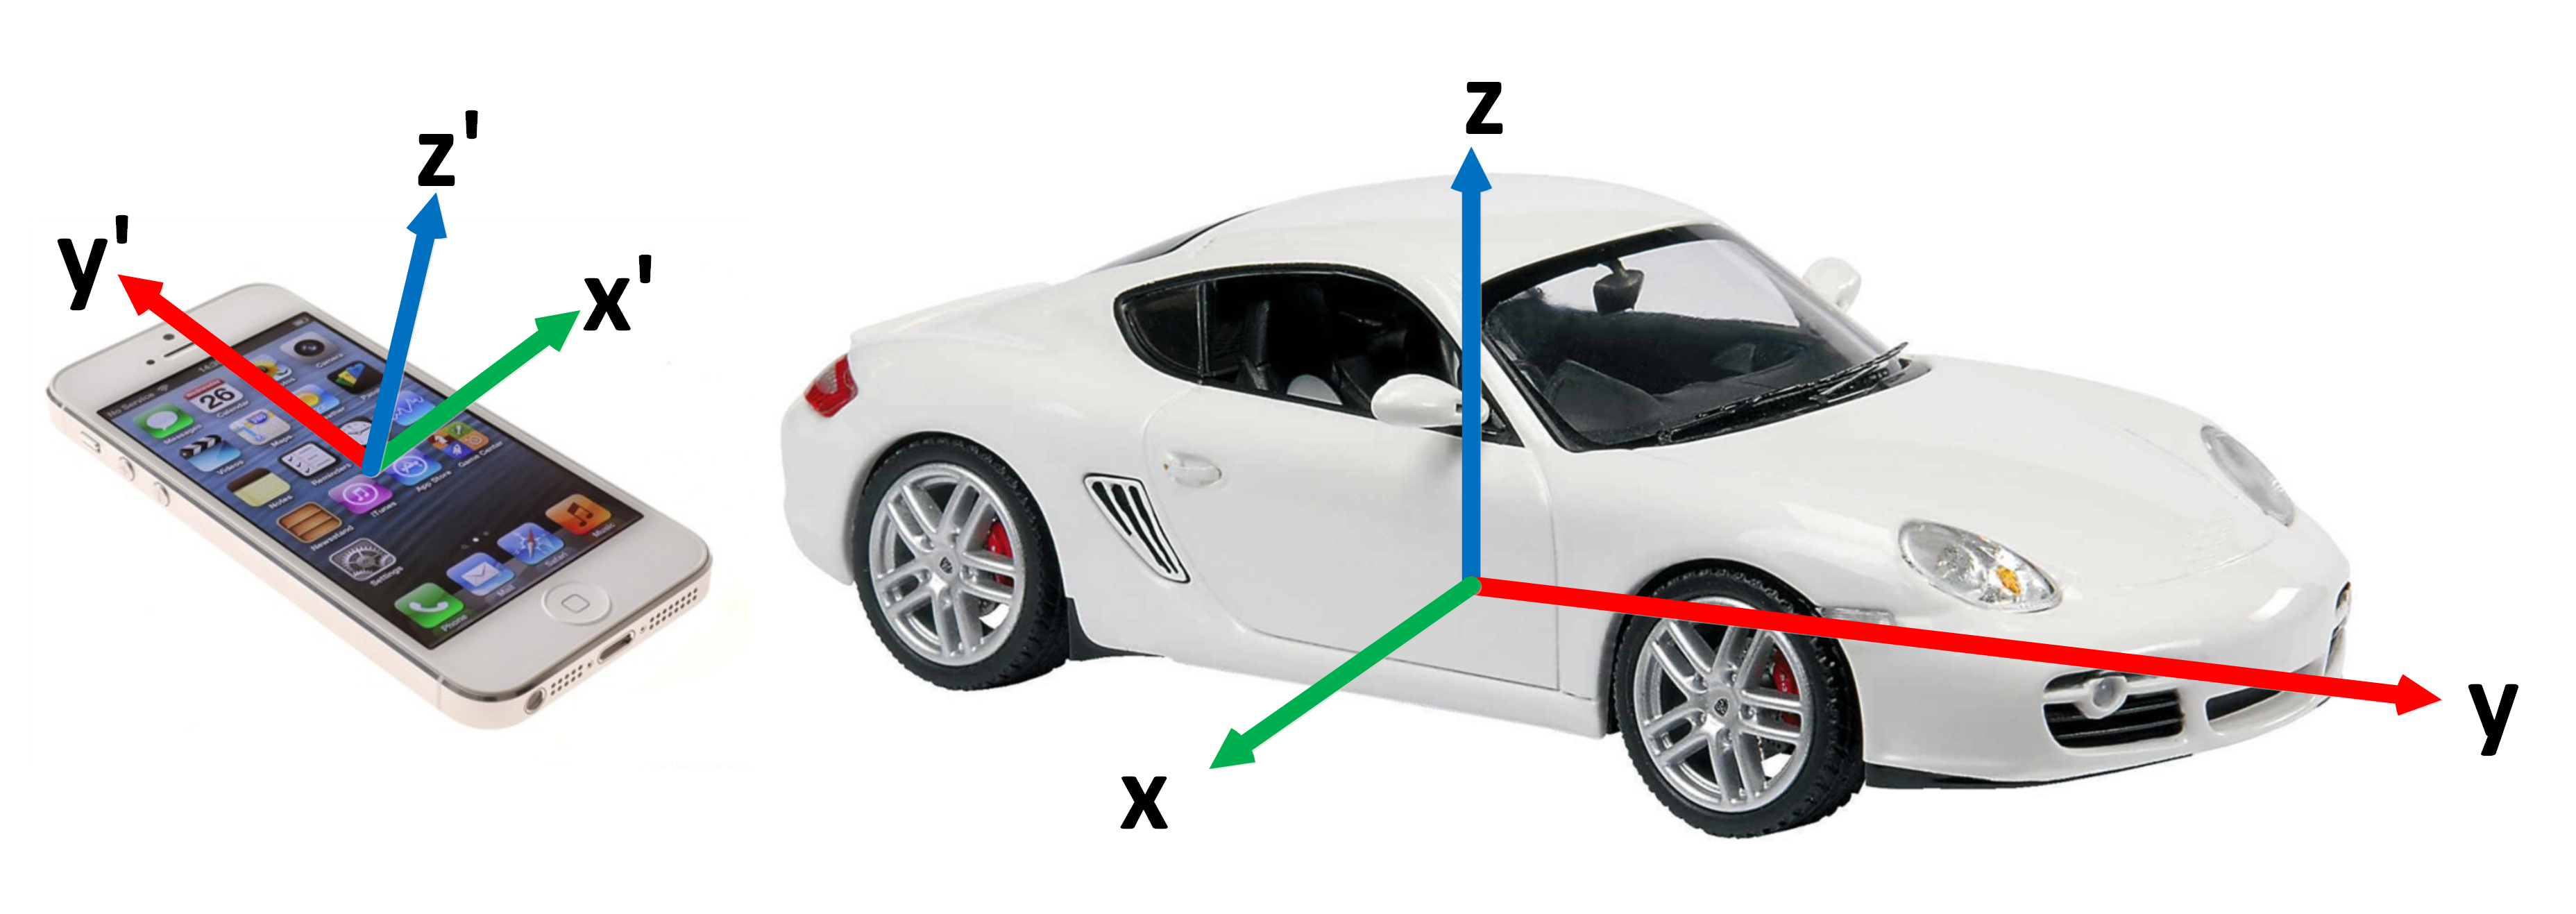
\includegraphics[width=0.5\textwidth]{coordinates}\\
  \caption{Coordinate systems of a vehicle ($x,y,z$) and a smartphone ($x',y',z'$).}\label{pix:coordinates}
\end{figure}

\subsection{Z-axis Estimation}% and Euler Angles Conversion}
The z-axis of the vehicle and the gravity are on exact opposite directions when the vehicle is on level ground. Thus we can tell the z-axis direction from that of the gravity. When the phone remains static or moves at constant speed, the only force and thus acceleration on the phone is the gravity. When the phone has other acceleration, various techniques can be used~\cite{Wang:2013_Driver_Phone_Use} to extract the components of the gravity on the phone's three axes at reasonable accuracy (e.g., iOS has an API to obtain those three components). Since vehicle movements will cause small, random disturbances on $x$ and $z$ axes acceleration even when moving along level, straight lines, we further average the extracted gravity samples within a time window. Thus such disturbances cancel out themselves on opposite directions of the same axis.

% However, the inertial sensor data of the smartphone's coordinate system may deviate from the real gravity direction because of the movement of the vehicle. To reduce this error, we averages inertial sensor data in a sliding time window and regard this as the gravity direction in the smartphone's coordinate system.

Given the z-axis direction in the phone's coordinate system, the angle the vehicle makes a turn on the $xy$ plane can be derived from the gyroscope data of the phone after a transformation. Thus we can tell whether the vehicle is moving along straight lines or making a turn.

%of the vehicle, we can derive the orientation of the smartphone on the xy-plane of the vehicle in the smartphone's coordinate system, according to the gyroscope data. This orientation is also the vehicle's orientation on its xy-plane if the smartphone is relatively static to the vehicle.

\subsection{Moving Detection}
To estimate the y-axis direction, we need to detect wether the vehicle is moving after knowing that it is not making a turn. To this end, we calculate the variance of accelerometer readings on three axes of the smartphone's coordinate system averaged within a sliding window. Theoretically, the accelerometer readings remain unchanged and the variance is zero if the vehicle is static or moving at a constant speed along a straight line. In practice, due to inevitable vibrations, small accelerations always happen and the variance cannot be zero.
%the vehicle will have vibration that can be detected by the accelerometer even it's static (xx how can it vibrate when static??).
We set a threshold and consider the vehicle static if the variance is smaller than the threshold. We find that this works very well for moving detection. Figure~\ref{pix:move} shows the normalized variance distribution during static and moving states. We can see that the overlapping portion is small compared to total areas.

\begin{figure}[h]
  \centering
  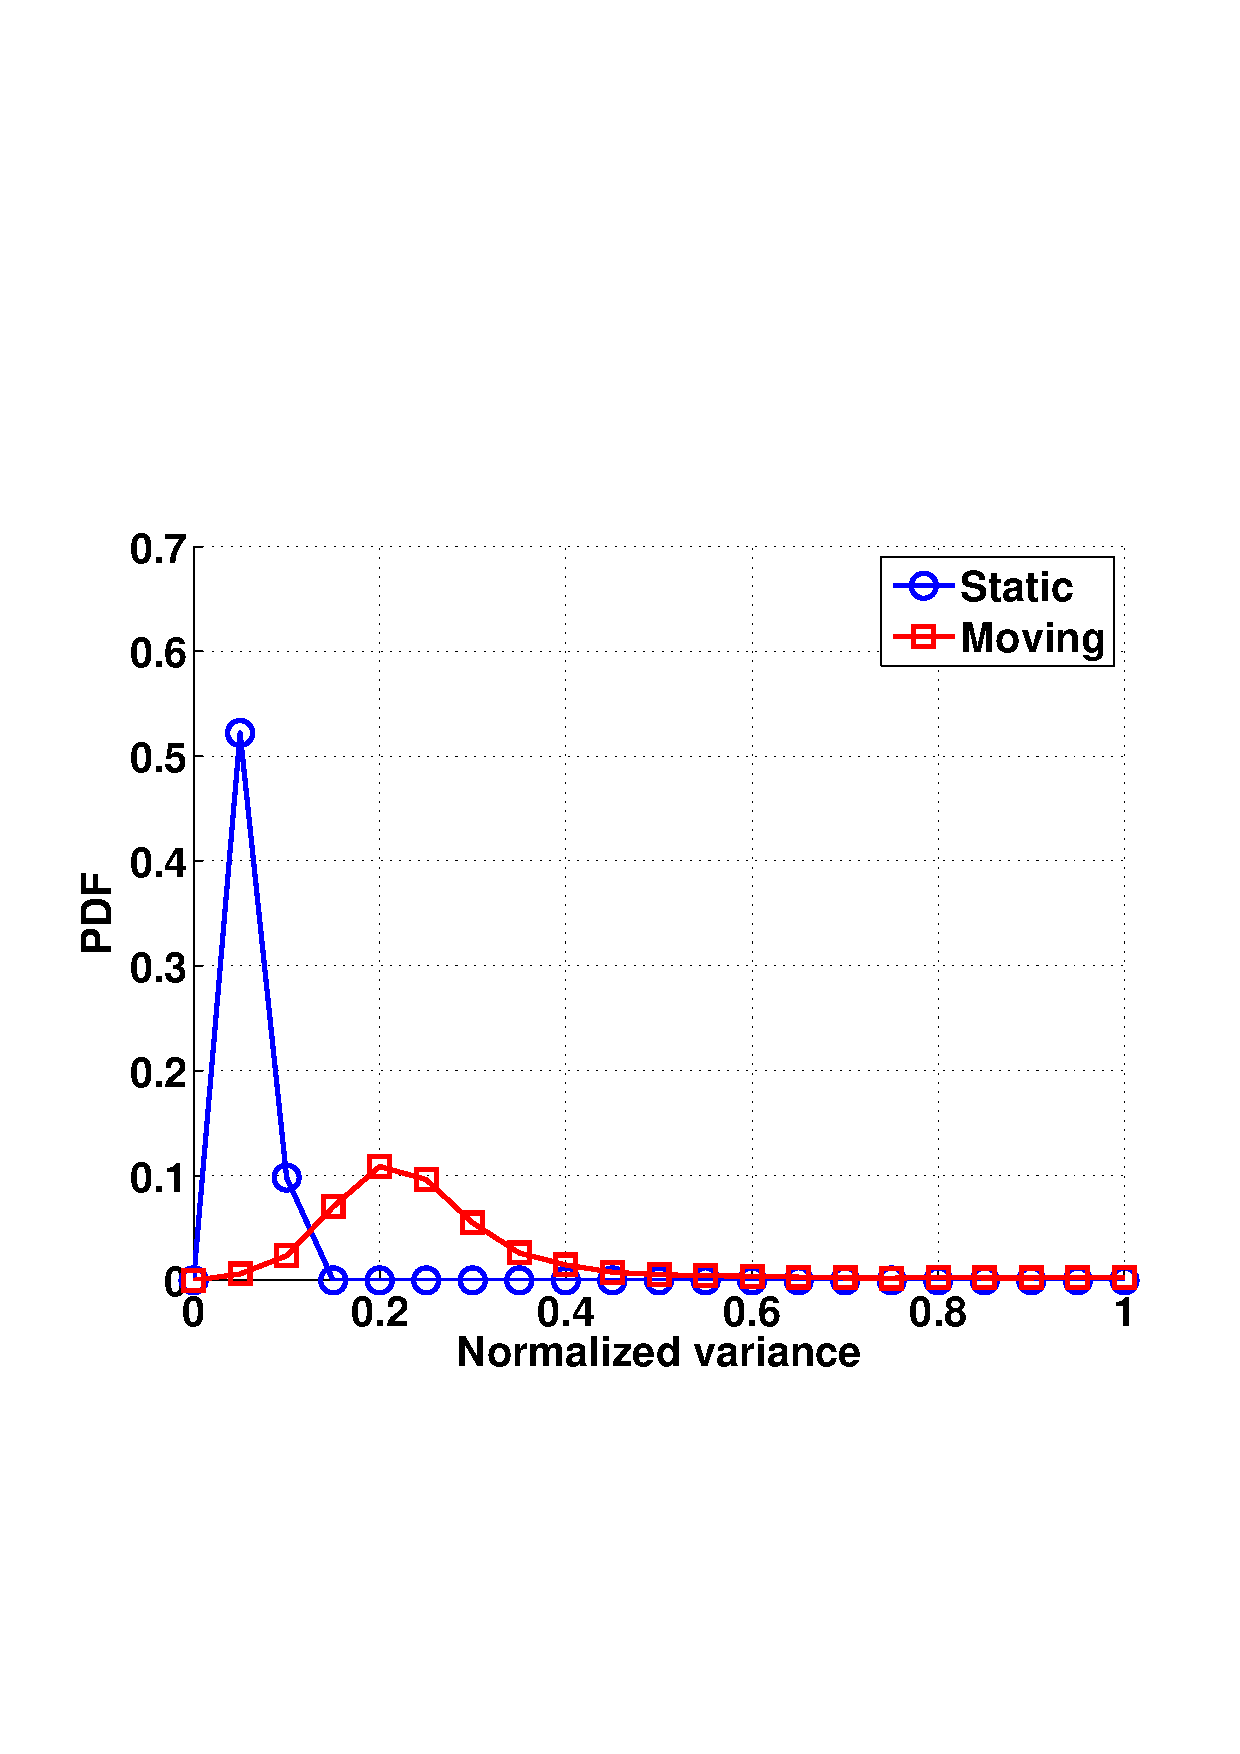
\includegraphics[width=0.35\textwidth]{move}\\
  \caption{Distribution of normalized standard deviation during static and moving states. }\label{pix:move}
\end{figure}

\subsection{Y-axis Direction Estimation} \label{subsec:pose_undirected}
Now we estimate the direction of the y-axis in the smartphone's coordinate system. During straight driving at constant speed, theoretically, the accelerometer readings are non-zero on the y-axis only (assuming gravity is removed). Thus the direction of acceleration is that of the $y$ axis in the phone's coordinate system. In practice, there are some noise on the x-axis because roads cannot be perfectly smooth.

Suppose that the direction of acceleration on the $xy$ plane is represented by a unit vector ${(cos\theta, sin\theta)}$ on the xy-plane of the vehicle. Given a set of accelerometer samples, we first project them onto the $xy$-plane of the vehicle. This can be done because the $z$ axis' direction is known. Denote the projected results ${(x_i,y_i), i = 1,...,k}$. We want to find the $\theta$ such that the total deviation of each of them from the true $y$ axis direction is minimized:
\begin{eqnarray}
&&\sum_{i=1}^{k}(x_icos\theta + y_icos\theta)^2\\
&=&asin2\theta + bcos2\theta + c\\
&=&\sqrt{a^2+b^2}sin(2\theta + \gamma) + c
\end{eqnarray}
where ${a=\sum_{i=1}^{k}x_i y_i}$,${b=\sum_{i=1}^{k}\frac{x_i^2-y_i^2}{2}}$,${c=\sum_{i=1}^{k}\frac{x_i^2+y_i^2}{2}}$,${tan\gamma=\frac{b}{a}}$.

This equation has a closed-formed solution:
\begin{equation}
\theta_1 = \frac{1}{4}\pi -  \frac{\gamma}{2}~~~~\theta_2 = \frac{5}{4}\pi - \frac{\gamma}{2}
\end{equation}
In the solution, we can see that there are two optimal solutions to ${\theta}$, representing the forward and backward directions of the vehicle, denoted by $\theta_1$ and $\theta_2$. Next we decide which is the true direction of the y-axis of the vehicle (i.e., the forward direction).

\subsection{Forward Direction Estimation} \label{subsec:pose_directed}
%(xx this part is very difficult to follow even after my revision. Someone familiar with the process should do another pass!!)

First we suppose that $\theta_1$ is the correct direction. Then we can get the estimated $(x, y, z)$ directions in the smartphone's coordinate system and project acceleromater readings to this coordinate system of the vehicle. In a short time period when the vehicle starts moving from static, there should be more positive acceleration on the y-axis direction.

We use a sliding time window starting at the beginning of the trace. Once we detect that the vehicle starts moving in this time window, we calculate the proportion of positive accelerometer readings within this time window such as:
\begin{equation}
\rho = \frac{1}{k}\sum_{i=1}^{k}y_i^3
\end{equation}
We use cubic form rather than linear form to better filter small noises caused by vibration of the vehicle, and focus on the real accelerometer readings caused by the acceleration of the vehicle.

% representing the forward and backward directions of the vehicle, denoted by $\theta_1$ and $\theta_2$.

However, this value is insufficient to determine whether $\theta_1$ or $\theta_2$ is the correct direction. Then, we put this value into sigmoid function and derive a probability of how $\theta_1$ likely equals $\theta$:
\begin{equation}
p(\theta=\theta_1)=\frac{1}{1+e^{-\rho}}
\end{equation}
The particle filter (in Section~\ref{sec:tracking}) then uses this probability as a prior to accurately converge on the correct direction---$\theta_1$ or $\theta_2$. This method helps narrow down the uncertainty caused by two opposite directions. % $\theta_1$ and $\theta_2$.





